% !TEX root=./report.tex

\section{Evaluation}

We assure the correctness and quantify the improvements resulting from the algorithms by an empirical study on the video streams of the highway cameras.

\subsection{Study Objects}
\begin{figure}[t]
    \begin{center}
    % \fbox{\rule{0pt}{2in} \rule{0.9\linewidth}{0pt}}
       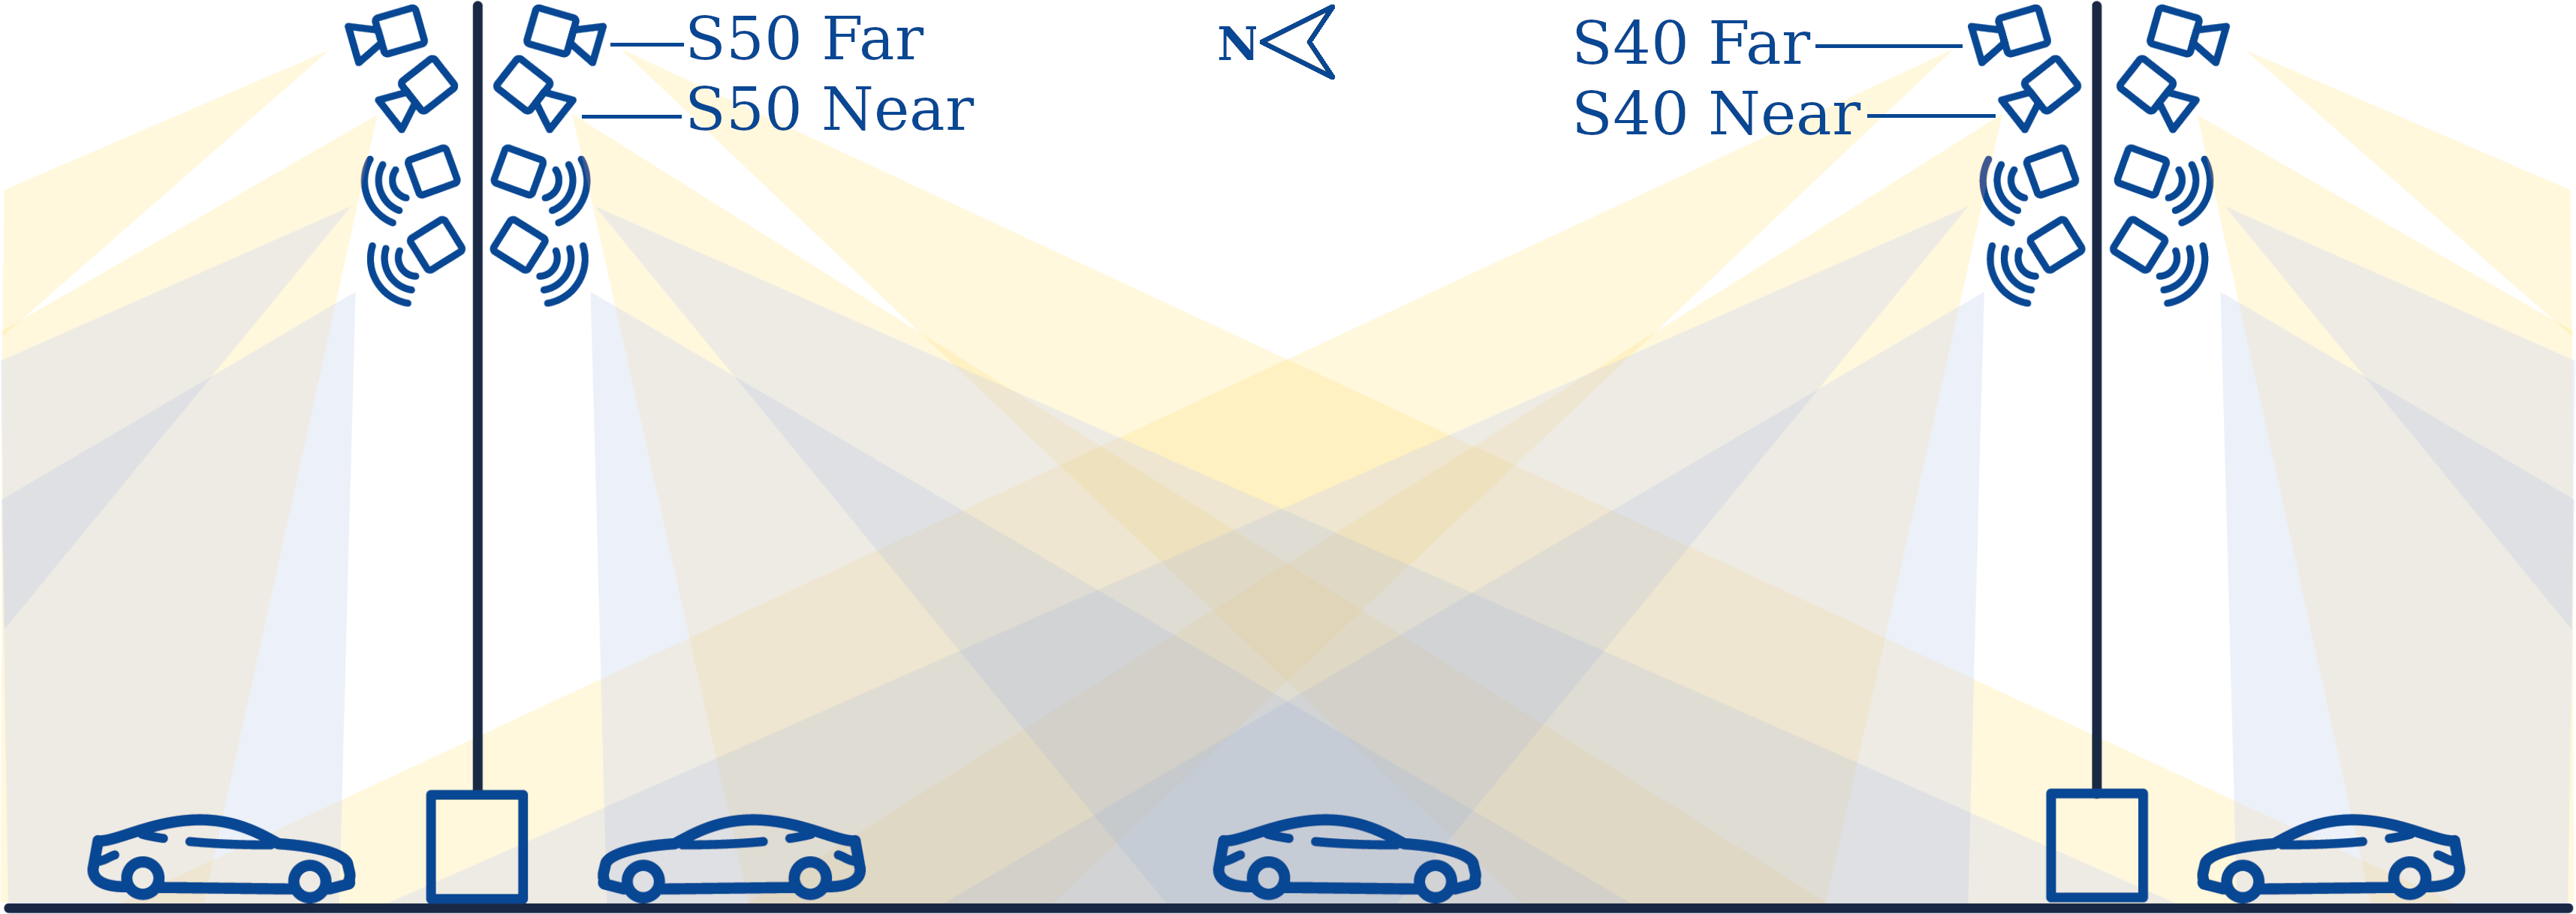
\includegraphics[width=\linewidth]{images/cameras_schema.png}
    \end{center}
       \caption{The schematic camera setup along the highway A9.
       The cameras \camsf{4} and \camsn{4} are facing north,
       the cameras \camsf{5} and \camsn{5} are facing south.}
    \label{fig:cameras_schema}
    \end{figure}

We use video recordings from the four cameras mounted to the two gantry bridges internally named S40 and S50. The schematic camera setup is displayed in \autoref{fig:cameras_schema}.

The dataset consists of four recordings, each with of a length of $1495$ frames over $\sim 60$ seconds at $25$ frames per second.
The recordings are taken on a day with strong winds to ensure high jitter in the video feed to optimally test the dynamic stabilization pipeline described in \autoref{sec:dynamic_stabilization_approach}. 

%%%%%%%%%%%%%%%%%%%%%%%%%%%%%%%%%%%%%%%%%%%%%%%%%%%%%%%%%%%%%%%%%%%%%%%%%%%%%%%%%%%%%%%%%%%%%%%%%%%%%%%%%%%%%%%%%%%%
%%%%%%%%%%%%%%%%%%%%%%%%%%%%%%%%%%%%%%%%%%%%%%%%%%%%%%%%%%%%%%%%%%%%%%%%%%%%%%%%%%%%%%%%%%%%%%%%%%%%%%%%%%%%%%%%%%%%
%%%%%%%%%%%%%%%%%%%%%%%%%%%%%%%%%%%%%%%%%%%%%%%%%%%%%%%%%%%%%%%%%%%%%%%%%%%%%%%%%%%%%%%%%%%%%%%%%%%%%%%%%%%%%%%%%%%%

\subsection{Dynamic Stabilization}
\label{sec:evaluation_dynamic_stabilization}
We evaluate and compare three pipeline instances based on the SURF \cite{bay10.1007/11744023_32,opencv_library} feature detector (SURF), 
ORB \cite{rublee6126544, opencv_library} feature detector (ORB) and FAST \cite{Ghahremani_2021,opencv_library} feature detector with FREAK \cite{alahi6247715,opencv_library} feature descriptors (FAST) 
and present two measures to evaluate the dynamic stabilization pipeline described in \autoref{sec:dynamic_stabilization_approach}.

%%%%%%%%%%%%%%%%%%%%%%%%%%%%%%%%%%%%%%%%%%%%%%%%%%%%%%%%%%%%%%%%%%%%%%%%%%%%%%%%%%%%%%%%%%%%%%%%%%%%%%%%%%%%%%%%%%%%
%%%%%%%%%%%%%%%%%%%%%%%%%%%%%%%%%%%%%%%%%%%%%%%%%%%%%%%%%%%%%%%%%%%%%%%%%%%%%%%%%%%%%%%%%%%%%%%%%%%%%%%%%%%%%%%%%%%%
%%%%%%%%%%%%%%%%%%%%%%%%%%%%%%%%%%%%%%%%%%%%%%%%%%%%%%%%%%%%%%%%%%%%%%%%%%%%%%%%%%%%%%%%%%%%%%%%%%%%%%%%%%%%%%%%%%%%

\subsubsection{Optical Flow}
\begin{figure*}[!ht]
    \centering
    \begin{tabular}{c}
      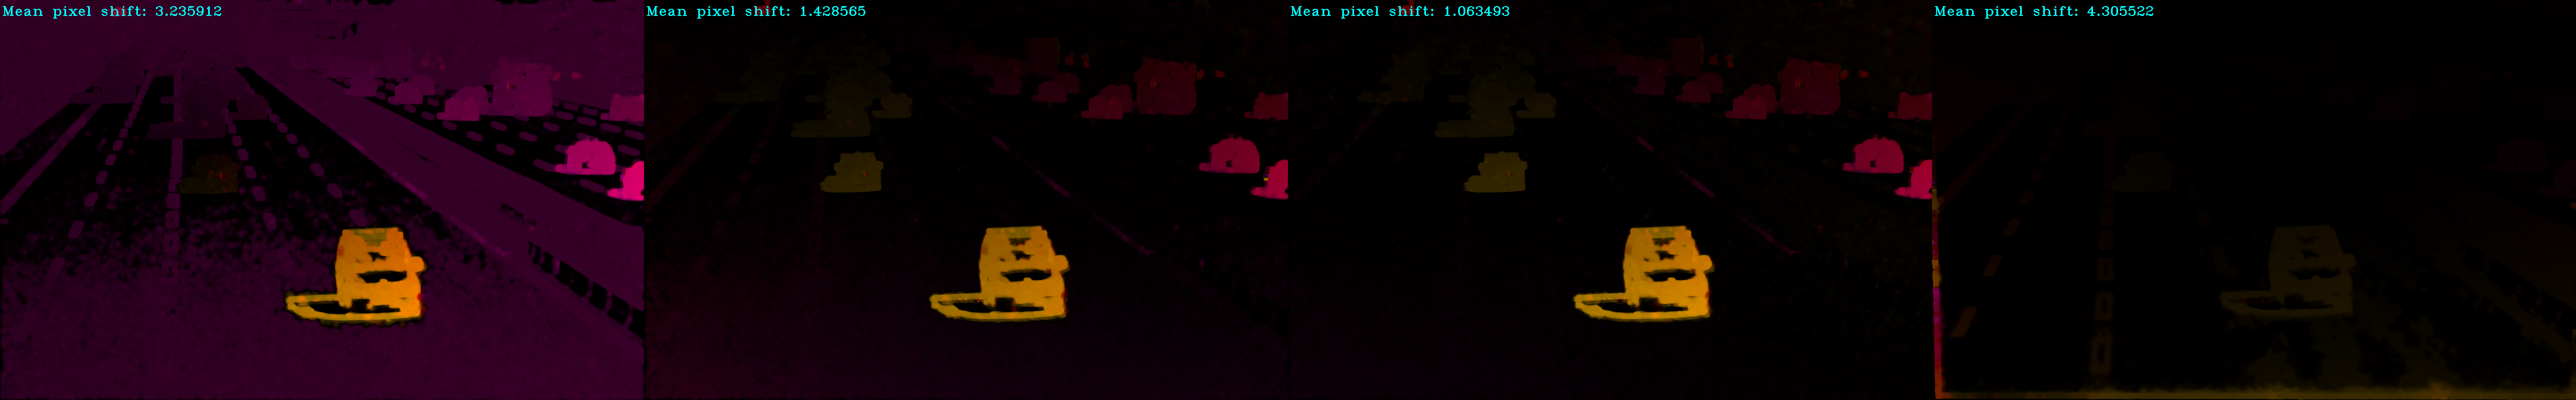
\includegraphics[width=0.95\linewidth]{images/frame_1317_cropped.png}    
    \end{tabular}
    \caption{
        From left to right: Original frame, stabilized using SURF, ORB and FAST.
        The dense optical flow displays the pixel displacement, the lighter the color the further the displacement. 
        The angle of displacement is color coded according to the HSV color circle.  
        In the original frame the violet background color indicates a jittery camera movement. 
        The car in the lower half is driving in the opposite direction as the camera jitters. 
    }
    \label{fig:optical_flow_example}
\end{figure*}

The optical flow is a 2D vector field where each vector is a displacement vector showing the movement of points between frames caused by movement of the objects or cameras.
It describes the apparent motion of image objects between two consecutive frames. 

We use the dense optical flow estimation algorithm proposed by Farnebäck \cite{farnback10.1007/3-540-45103-X_50,opencv_library} to measure the displacement of each pixel between the frames. 
We calculate the mean displacement over the whole image to get the overall displacement. 

\autoref{fig:optical_flow_example} displays one frame of optical flow calculated pre and after stabilization.
It qualitatively shows that the static background scene is dark in the stabilized frames which indicates a low optical flow and thus nearly no movement. 
We see a car driving, indicated by the yellow patch, that remains as expected using SURF and ORB, but gets filtered out by FAST. This problem is described in \autoref{sec:dynamic_stabilization_evaluation_optical_flow_problem}.     

\begin{figure}[t]
    \centering
    \begin{tabular}{c}
      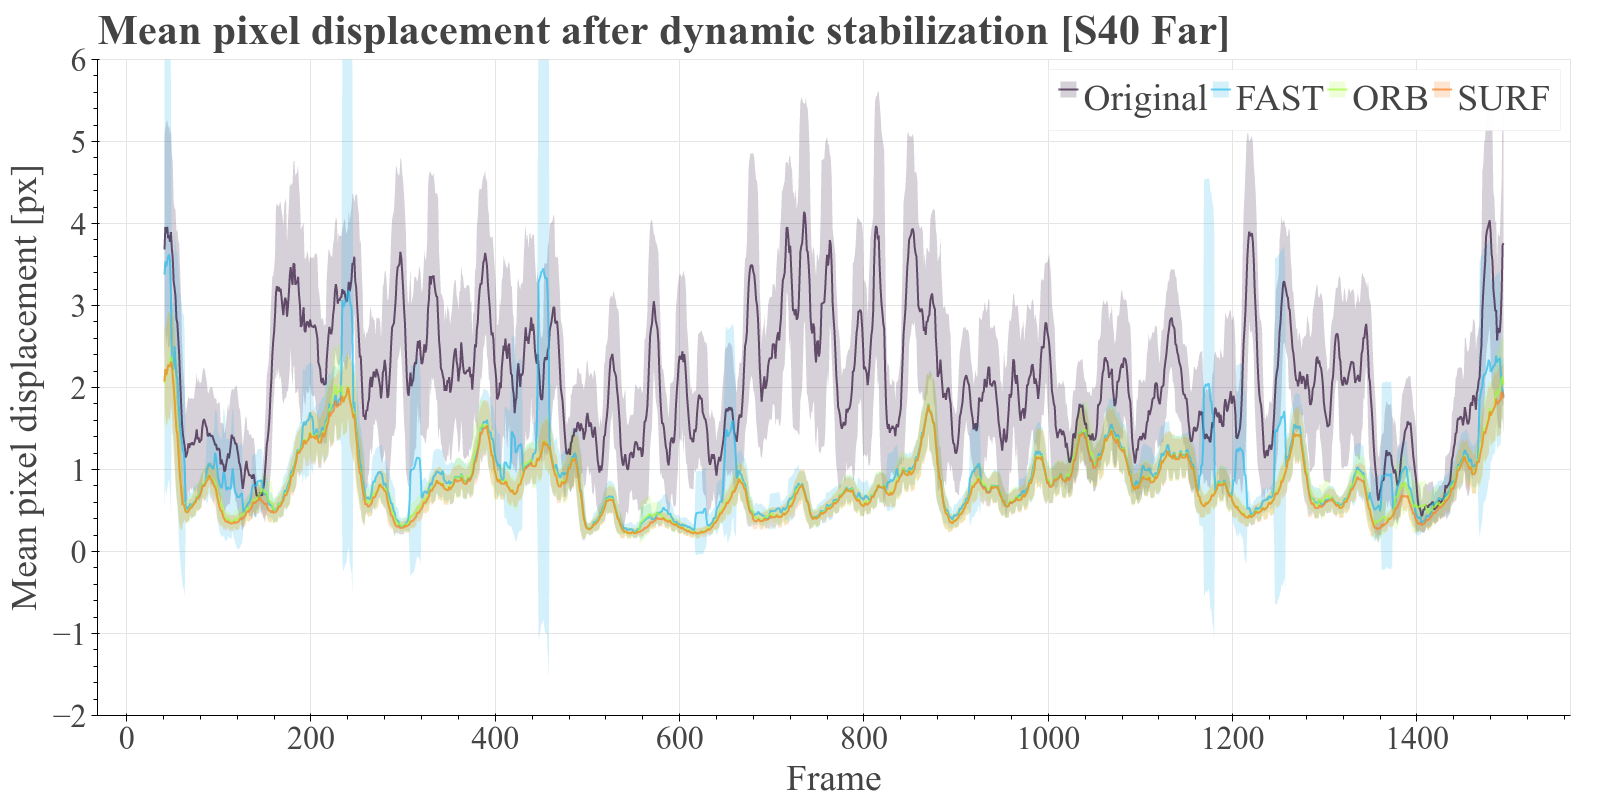
\includegraphics[width=0.9\linewidth]{diagrams/optical_flow/mean_pixel_shifts_after_dynamic_stabilization_s40_far.png}    \\  
      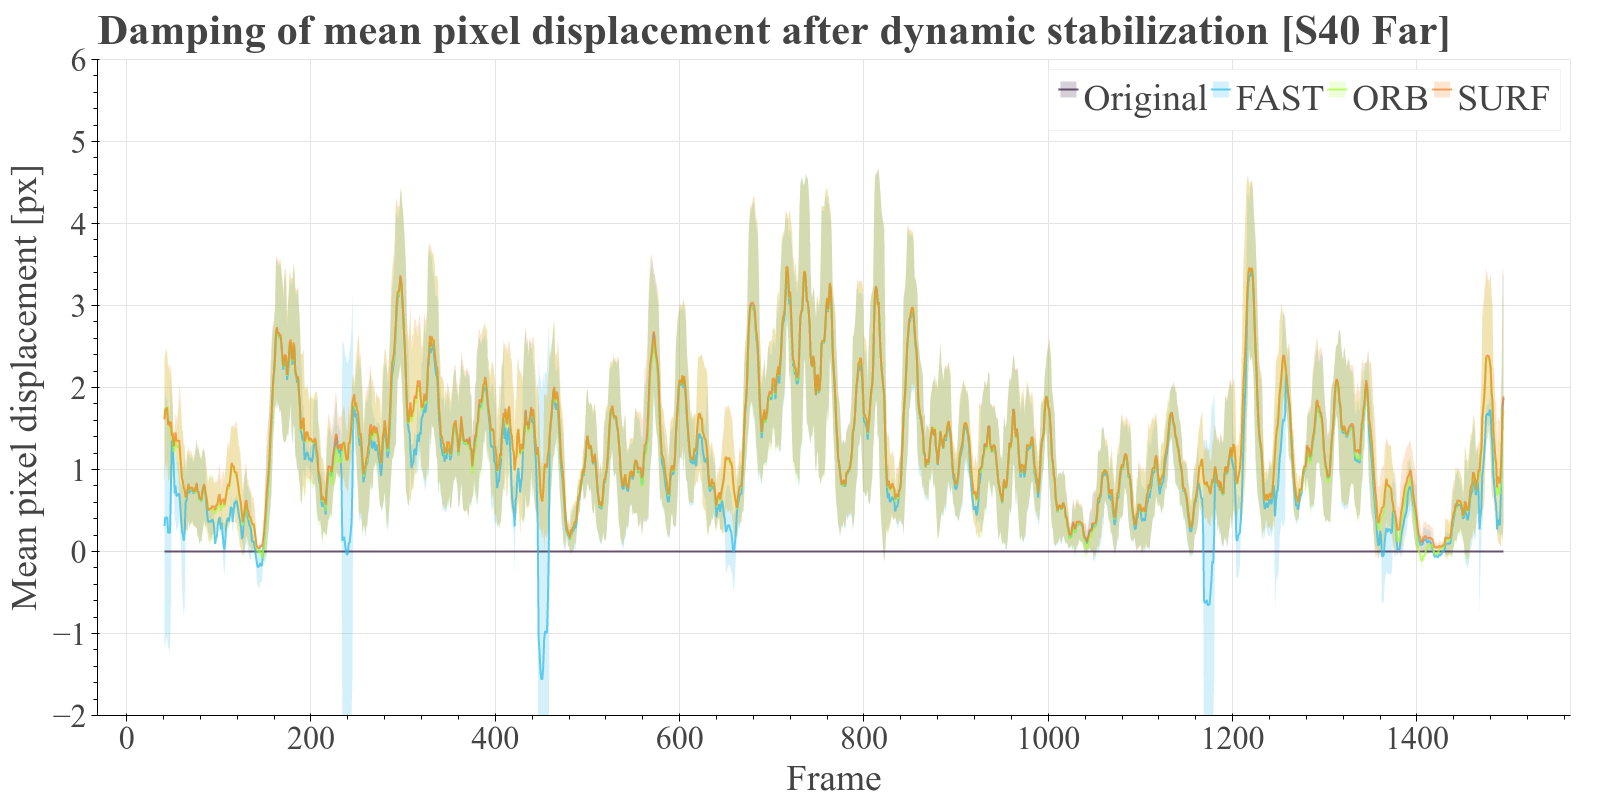
\includegraphics[width=0.9\linewidth]{diagrams/optical_flow/damping_mean_pixel_shifts_after_dynamic_stabilization_s40_far.png}    
\end{tabular}
    \caption{Top: 
        Comparison of the three implemented dynamic stabilizers (SURF, ORB, FAST) and the original not stabilized video feed using optical flow as measure (lower is better).
        The graphs display the mean pixel shift at each frame. 
        Bottom: 
        The damping capabilities of the same three stabilizers (higher is better). 
        The graphs approximate the removed jitter in the mean pixel shift between the original video and the stabilizer at each frame.\\
        For visualization the values are filtered using the rolling mean over 12 frames. 
        The light areas display the standard deviation within the window.
    }
    \label{fig:dynamic_stabilization_s40_far}
\end{figure}

\autoref{fig:dynamic_stabilization_s40_far} displays the mean pixel displacement (MPD) per frame calculated as the mean of the lengths of the vectors in the optical flow field and the damping as the difference of the mean displacements over the original and stabilized frame.
It shows that the original frames have a MPD of up to $5$ pixels per frame. This implies that on average every pixel on the dynamic scene and static background had moved by $5$ pixels per frame. 
The displacement is damped by all of the stabilizers by a mean of up to $4.5$ pixels, whereas the remaining displacement is due to the actually moving vehicles in the dynamic foreground.   

\begin{figure}[!ht]
      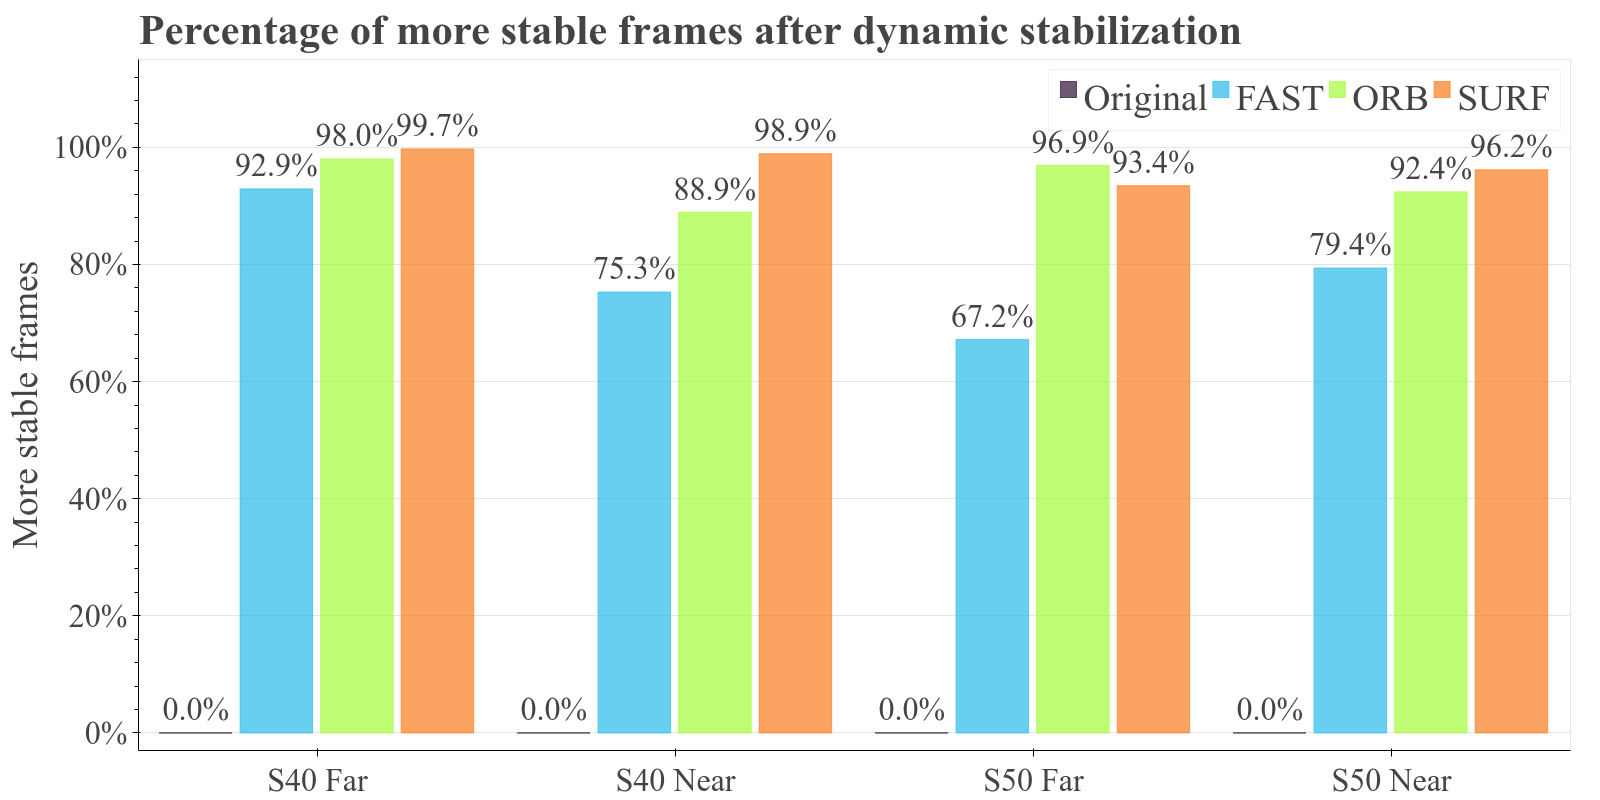
\includegraphics[width=\linewidth]{diagrams/optical_flow/stats.png}    
    \caption{
        Comparison of the percentages of more stable frames after dynamic stabilization per camera and stabilizer.
        A frame is classified as more stable if the MPD is lower than for the original video feed. 
    }
    \label{fig:dynamic_stabilization}
\end{figure}

\autoref{fig:dynamic_stabilization} displays the percentage of frames that are more stable than the original frame.
We define a frame to be more stable if its MPD is lower than the MPD of the original frame. 
It shows that for SURF and ORB at least $88.9\%$ ranging up to $99.7\%$ of frames are more stable.
For the FAST detector it shows that except for the \camsf{4} camera only between $67.2\%$ to $79.4\%$ of frames are more stable, whereas a value of $50\%$ would indicate that the other $50\%$ of frames are worse.  


%%%%%%%%%%%%%%%%%%%%%%%%%%%%%%%%%%%%%%%%%%%%%%%%%%%%%%%%%%%%%%%%%%%%%%%%%%%%%%%%%%%%%%%%%%%%%%%%%%%%%%%%%%%%%%%%%%%%
%%%%%%%%%%%%%%%%%%%%%%%%%%%%%%%%%%%%%%%%%%%%%%%%%%%%%%%%%%%%%%%%%%%%%%%%%%%%%%%%%%%%%%%%%%%%%%%%%%%%%%%%%%%%%%%%%%%%
%%%%%%%%%%%%%%%%%%%%%%%%%%%%%%%%%%%%%%%%%%%%%%%%%%%%%%%%%%%%%%%%%%%%%%%%%%%%%%%%%%%%%%%%%%%%%%%%%%%%%%%%%%%%%%%%%%%%


\paragraph{Problem of Optical Flow as a Measure}
\label{sec:dynamic_stabilization_evaluation_optical_flow_problem}
Optical flow cannot distinguish between dynamically moving objects and static scene.
This is especially a problem when a jitter of the camera moves the pixels in the opposite direction as the vehicles path is pointing in image space.
This jitter blurs the movement of the dynamic objects into the background and thus removes some of the real movement.
The dynamic stabilization then reintroduces the real movement of the vehicle, thus showing some frames after stabilization to be worse than before. 

This should be taken with caution as the optical flow cannot detect the relative motion and thus is not a definite measure for the jitter.
Nonetheless, it hints at the overall stabilization capabilities of the presented pipeline, but cannot give a direct explanation for single worse frames.

%%%%%%%%%%%%%%%%%%%%%%%%%%%%%%%%%%%%%%%%%%%%%%%%%%%%%%%%%%%%%%%%%%%%%%%%%%%%%%%%%%%%%%%%%%%%%%%%%%%%%%%%%%%%%%%%%%%%
%%%%%%%%%%%%%%%%%%%%%%%%%%%%%%%%%%%%%%%%%%%%%%%%%%%%%%%%%%%%%%%%%%%%%%%%%%%%%%%%%%%%%%%%%%%%%%%%%%%%%%%%%%%%%%%%%%%%
%%%%%%%%%%%%%%%%%%%%%%%%%%%%%%%%%%%%%%%%%%%%%%%%%%%%%%%%%%%%%%%%%%%%%%%%%%%%%%%%%%%%%%%%%%%%%%%%%%%%%%%%%%%%%%%%%%%%


\subsubsection{Track features and calculate path smoothness}
We randomly took three sample vehicles per camera and tracked their pixel locations over the sequence.
As the vehicles move through the image the bounding box of the object is found using the \emph{Discriminative Correlation Filter With Channel and Spatial Reliability} proposed by Lukezic \etal{} \cite{Lukezic_2017_CVPR,opencv_library}.
The center point of the bounding box is then written to disk and used as the predicted pixel location $p$ of the vehicle.

We only track in the original frame to remove inaccuracies in the tracking and use the homographic transformation matrix from \autoref{eq:dynamic_stabilization_homographic_transformation} that stabilizes the frame to also stabilize the bounding box.
This gives us comparable results for the pixel locations. 

We calculate the travelled distance of the pixel locations of the objects as they move through the image. 
This distance is a direct measure for the jittery motion in the image as it introduces large jumps of the tracked positions, thus directly increasing the travelled distance.

The travelled distance is formulated as the arc length
\begin{equation}
    arc(vehicle) = \sum_{n = 1}^{\left\lvert frames \right\rvert } \left\lVert 
        p_{i} - p_{i-1}
    \right\rVert _2
\end{equation} 
based on the finite differences between consecutive tracked positions.
To get comparable results a normalization 
\begin{equation}
    narc_{stabilizer}(vehicle) = 
    \frac{arc_{stabilizer}(vehicle)}{arc_{original}(vehicle)}
\end{equation} 
is performed by the arc length of the original video frame.

\autoref{fig:object_tracking_s40_n_far} displays the vehicles tracked in the video sequence taken from the camera \camsf{4}. 
There is one red truck, a black pickup and a white car taken as random samples.
The tracking is performed als long as the vehicles are visible.
It shows that the travelled distances of the pixels after dynamic stabilization remain at between $43\%$ and $68.4\%$ compared to the original one.   
This implies that much of the additional motion introduced by the environmental influences are removed and the remaining path displays the real projected path of the vehicle. 

\begin{figure*}[!ht]
    \centering
    \begin{tabular}{cc}
      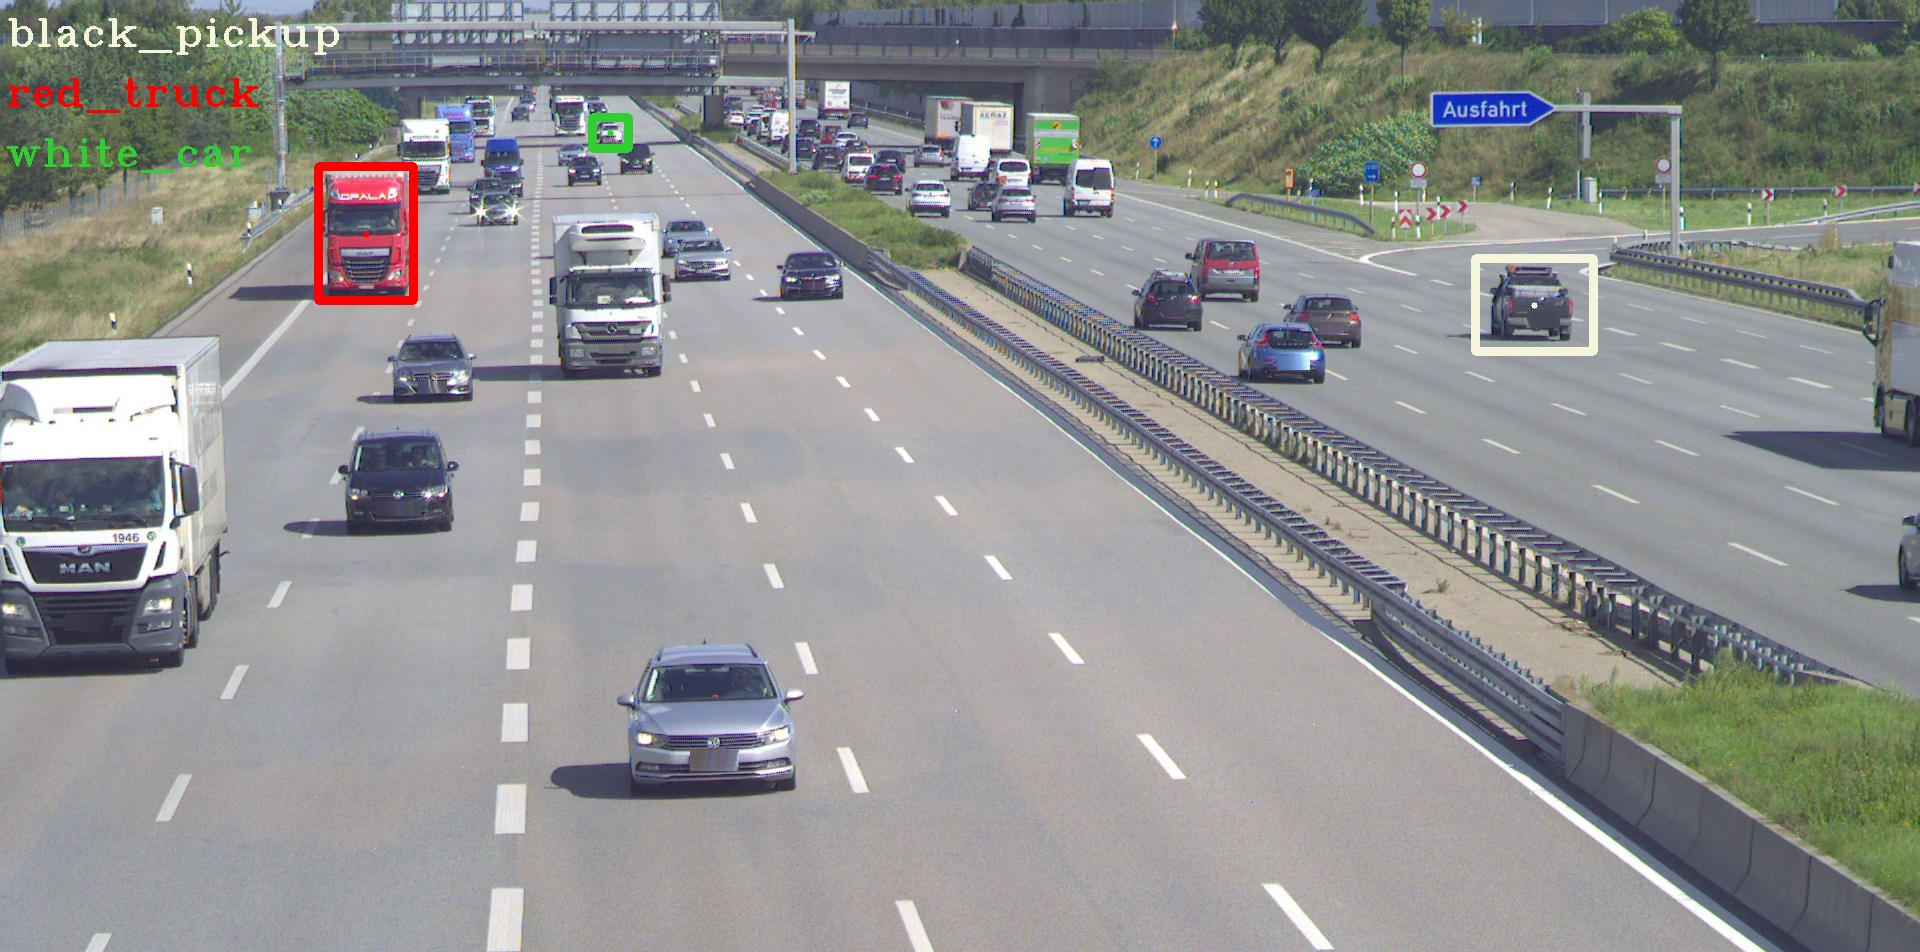
\includegraphics[width=0.475\linewidth]{diagrams/object_tracking/s40_n_far/frame_cropped.png}    &  
      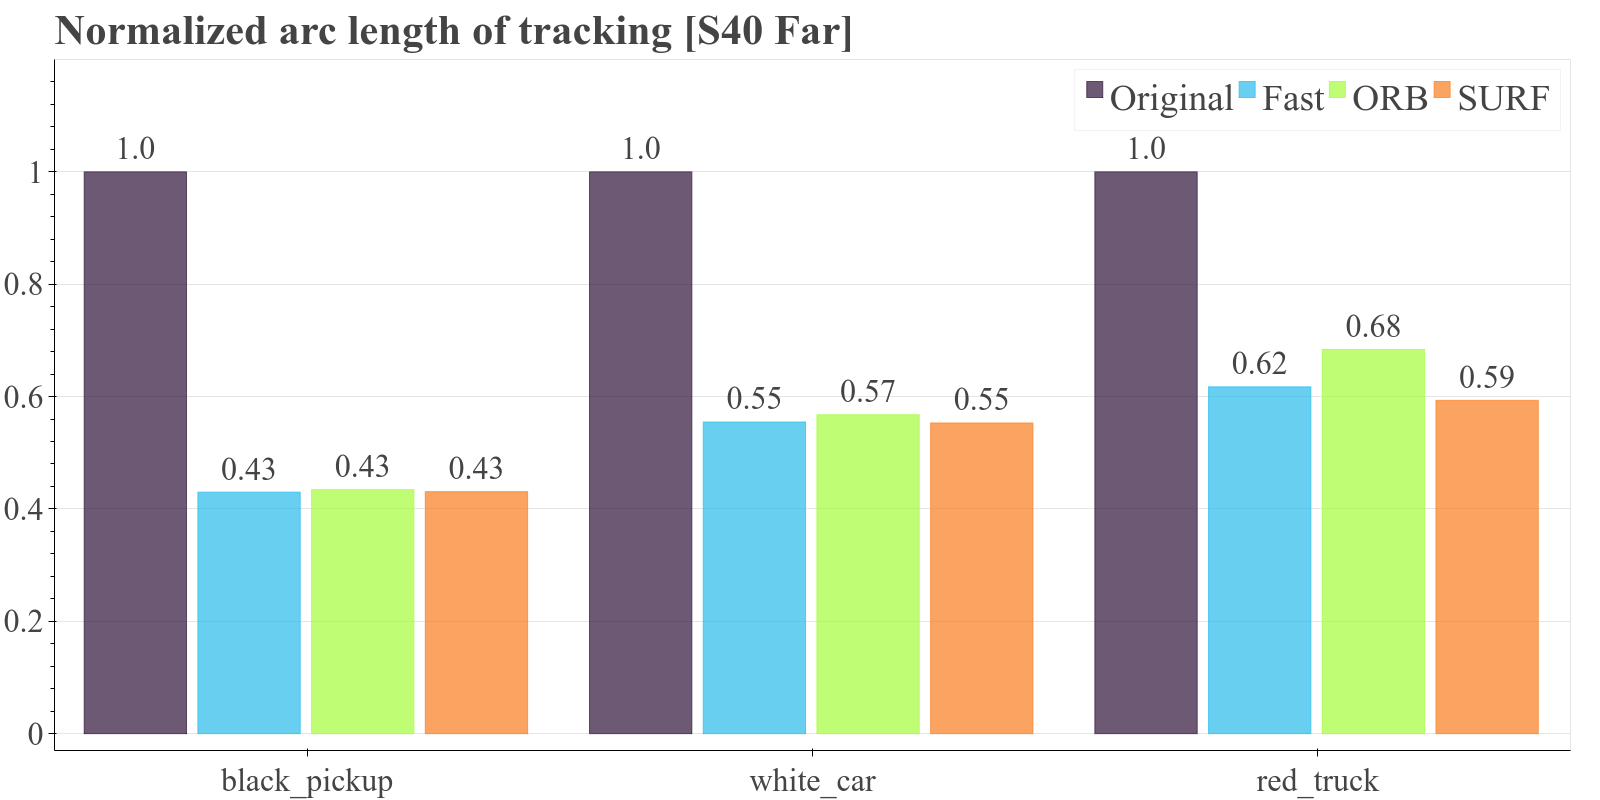
\includegraphics[width=0.475\linewidth]{diagrams/object_tracking/s40_n_far/arcs.png}    
    \end{tabular}
    \caption{Left: 
    The exemplary vehicles tracked through the video sequence of the camera \camsn{4}. 
    Right:
    The corresponding normalized arc lengths of the pixel path. 
    The removed jitter is directly proportional to the decrease in the normalized arc lengths, as the pixel only follows the real vehicles movement.
    }
    \label{fig:object_tracking_s40_n_far}
\end{figure*}

We included plots for the tracked pixel locations and the comparison of the arc lengths for the other three cameras in the Appendix (\autoref{sec:appendix}).

\subsubsection{Speed comparison}